\chapter{The Hiring Filter: Skills, Traits, and Early Team Judgment}

This chapter follows a short School of Hard Knocks entrepreneurship interview segment, curated by LazyingArt LLC through Video2Book, in which the central question is not how to admire talent from a distance, but how to decide who belongs on an early team. The answer unfolds in a simple order: first we recognize natural role fit, then we ask whether that fit is enough, and finally we arrive at the non-negotiable traits that make talent usable inside a venture.

\section{The Founder’s Selection Problem}

The opening question is a founder's question. When we are building a company or launching a venture, we are not merely collecting impressive people. We are deciding who can enter a small system where every person changes the motion of the whole firm.

Let \(c\) denote a candidate for the team. The first object of judgment is not yet character, and not yet credentials. It is the candidate's apparent operating lane:
\begin{equation}
  c \longmapsto \operatorname{RoleType}(c).
\end{equation}
In the interview, the examples are concrete: a sales type, an engineering type, and an operations type. These are not formal categories. They are founder shorthand for where a person appears naturally strong.

We can write the first screen as:
\begin{equation}
  \operatorname{RoleType}(c) \in
  \{\text{sales},\ \text{engineering},\ \text{operations},\ \ldots\}.
\end{equation}
This is useful information, but it is deliberately not the end of the argument. The speaker grants that people have things they are naturally good at, and then pivots to the more important distinction.

\section{Natural Role Fit Is Only the First Signal}

A candidate's role type tells us where the person may contribute. It does not tell us whether the person can be built with. That is the difference between a job label and a team decision.

For an early company, role fit is a necessary kind of evidence:
\begin{equation}
  \operatorname{Hire}(c) \Rightarrow \operatorname{RoleFit}(c)
  \quad\text{is plausible,}
\end{equation}
but the reverse implication is too strong:
\begin{equation}
  \operatorname{RoleFit}(c) \nRightarrow \operatorname{Hire}(c).
\end{equation}
The lecture's rhythm matters here. The answer does not begin by dismissing skill. It first accepts that skill and natural lane are visible. Only after that does it ask what those signals fail to prove.

\subsection{Question \& Answer}

\paragraph{Question.}
If someone is visibly talented, or clearly belongs to a useful role type, is that enough reason to bring the person onto the team?

\paragraph{Answer.}
No. The speaker's answer is that skill can be taught, but traits cannot be reliably installed from the outside. A talented person may still fail inside this company if the deeper operating traits are missing.

In compact form, the claim is:
\begin{equation}
  \text{skill is trainable}
  \qquad\text{but}\qquad
  \text{traits are non-negotiable}.
\end{equation}
This is not presented as a psychological theorem. It is a founder's hiring rule, stated from practical experience.

\section{The Trainable Skill and Fixed Trait Distinction}

The pivot phrase in the interview is essentially, ``at the end of the day.'' That is where we move from role classification to the deeper hiring constraint.

Let \(S(c)\) stand for the candidate's current skill level, and let \(T(c)\) stand for the candidate's relevant trait profile. The speaker treats these differently:
\begin{align}
  S(c) &\longrightarrow S(c) + \Delta S
  \quad\text{through teaching, practice, and management},\\
  T(c) &\not\longrightarrow T(c) + \Delta T
  \quad\text{by ordinary workplace instruction}.
\end{align}
This notation is only a clean reconstruction of the spoken idea. It captures the asymmetry: skills can move under training, but the traits that make training work must already be present in some meaningful degree.

A simple update rule for a teachable skill is:
\begin{equation}
  S_{t+1}(c)=S_t(c)+\Delta S_t(c),
  \qquad \Delta S_t(c)>0
  \quad\text{when the person can learn}.
\end{equation}
But the condition ``when the person can learn'' is doing the real work. Coachability and humility are not decorative virtues in this passage. They are the conditions that allow the skill update to happen.

\section{The Non-Negotiable Trait Set}

The speaker then names the filter. Talent, school, and referrals are explicitly demoted. The traits that matter are coachability, humility, and persistence.

We can collect the stated non-negotiables as:
\begin{equation}
  \mathcal{T}
  =
  \{\text{coachable},\ \text{humble},\ \text{persistent}\}.
\end{equation}
A candidate clears the trait screen only if all three conditions are present:
\begin{equation}
  \operatorname{TraitClear}(c)
  =
  \operatorname{Coachable}(c)
  \land
  \operatorname{Humble}(c)
  \land
  \operatorname{Persistent}(c).
\end{equation}
The point is not that these are the only virtues in business. The point is narrower and more useful: in this interview, these are the speaker's non-negotiables for deciding whether a talented person can actually become useful inside the company.

\begin{table}
\centering
\begin{tabular}{|p{0.24\linewidth}|p{0.31\linewidth}|p{0.31\linewidth}|}
\hline
Signal & What it may show & What it does not prove \\
\hline
Sales, engineering, or operations type & A natural lane for contribution & That the person can learn inside this firm \\
\hline
Talent & Existing ability or performance & That the person is coachable or humble \\
\hline
School or referral & A credential or social signal & That the person will persist here \\
\hline
\end{tabular}
\end{table}

\section{A Compact Hiring Filter}

The lecture's reasoning can be redrawn as a narrow decision path. This is not a screenshot reconstruction; no validated board or diagram image is available for this interview segment. It is a transcript-derived map of the spoken hiring logic.

\begin{figure}
\centering
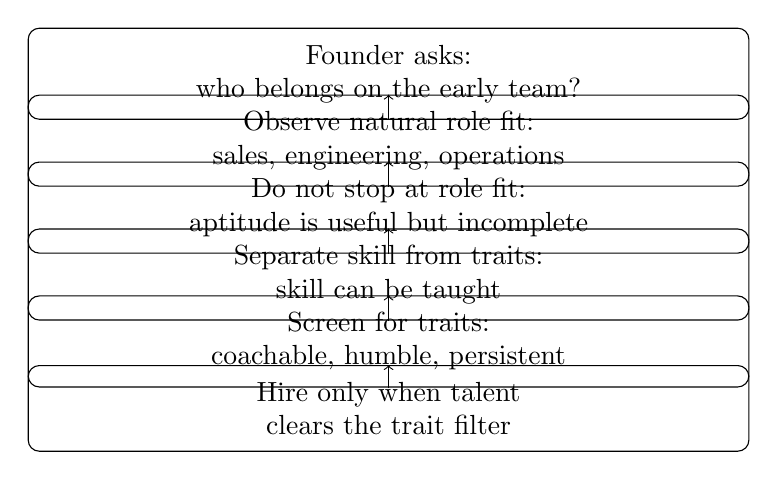
\begin{tikzpicture}[
  node distance=0.85cm,
  every node/.style={
    draw,
    rounded corners,
    align=center,
    text width=0.72\linewidth,
    inner sep=6pt
  },
  every path/.style={->}
]
\node (q) {Founder asks:\\ who belongs on the early team?};
\node (role) [below of=q] {Observe natural role fit:\\ sales, engineering, operations};
\node (limit) [below of=role] {Do not stop at role fit:\\ aptitude is useful but incomplete};
\node (skill) [below of=limit] {Separate skill from traits:\\ skill can be taught};
\node (traits) [below of=skill] {Screen for traits:\\ coachable, humble, persistent};
\node (hire) [below of=traits] {Hire only when talent\\ clears the trait filter};

\draw (q) -- (role);
\draw (role) -- (limit);
\draw (limit) -- (skill);
\draw (skill) -- (traits);
\draw (traits) -- (hire);
\end{tikzpicture}
\end{figure}

In formula form, the reconstructed rule is:
\begin{equation}
  \operatorname{Hire}(c)
  \Rightarrow
  \operatorname{RoleFit}(c)
  \land
  \operatorname{TraitClear}(c).
\end{equation}
The speaker's emphasis is even stronger than this implication. The practical decision rule is closer to:
\begin{equation}
  \operatorname{RoleFit}(c)
  \land
  \operatorname{TraitClear}(c)
  \longrightarrow
  \text{candidate worth serious consideration}.
\end{equation}
Role fit opens the door. Trait fit decides whether the door should remain open.

\section{Worked Example: The Talented Sales Rep}

The interview closes the point with a concrete case. Suppose \(c\) is a strong sales representative at some outside company, called generically ``XYZ company'' in the transcript. We observe:
\begin{equation}
  \operatorname{Talent}(c)=1,
  \qquad
  \operatorname{RoleType}(c)=\text{sales}.
\end{equation}
That is good evidence. It says the person can probably sell. But the speaker says it still does not imply success here:
\begin{equation}
  \operatorname{Talent}(c)
  \lor
  \operatorname{School}(c)
  \lor
  \operatorname{Referral}(c)
  \nRightarrow
  \operatorname{SuccessHere}(c).
\end{equation}

The worked hiring check therefore runs in order:
\begin{enumerate}
  \item Identify the visible role strength:
  \[
    \operatorname{RoleType}(c)=\text{sales}.
  \]
  \item Acknowledge existing talent:
  \[
    \operatorname{Talent}(c)=1.
  \]
  \item Test whether the person is coachable:
  \[
    \operatorname{Coachable}(c)=1?
  \]
  \item Test whether the person is humble:
  \[
    \operatorname{Humble}(c)=1?
  \]
  \item Test whether the person is persistent:
  \[
    \operatorname{Persistent}(c)=1?
  \]
\end{enumerate}
Only when those tests clear does talent become a useful asset for the venture. Without them, talent remains merely an external signal.

\section{Summary}

The interview gives a compact theory of early-team selection. First, notice what people are naturally good at: sales, engineering, operations, or another role lane. Then refuse to confuse visible ability with complete evidence. The decisive distinction is between skill, which can be taught, and traits, which the speaker treats as non-negotiable.

The final hiring filter is therefore simple but demanding:
\begin{equation}
  \boxed{
  \operatorname{Hire}(c)
  \text{ only after }
  \operatorname{RoleFit}(c)
  \text{ and }
  \operatorname{TraitClear}(c)
  }
\end{equation}
For this speaker, the traits that make the filter work are coachability, humility, and persistence. Talent matters, but it matters after those conditions are met.